\documentclass{article}
\usepackage{polski}
\usepackage{blindtext}
\usepackage{amsmath}
\usepackage{mathtools}
\usepackage{graphicx} 
\usepackage[a4paper, left=2.5cm, right=2.5cm, top=3.5cm, bottom=3.5cm, headsep=1.2cm]{geometry}




\title{\textsc{Sprawozdanie - laboratorium 1}}


\date{Zuzanna Grzesik, 25.02.2020}
\author{\Large{\textbf{Rozwiązywanie UARL metodami bezpośrednimi}}}


\begin{document}
\maketitle

	
\section{Wstęp teoretyczny}	
\par	
Na laboratorium zajęliśmy się tematem układów algebraicznych równań liniowych i rozwiązywaniu ich metodami bezpośrednimi. 
Układy równań liniowych możemy zapisać również w postaci macierzowej, a~dzięki tej postaci możemy skorzystać z innych metod rozwiązywania układu, np. metody Gaussa-Jordana.
\subsection{Metoda Gaussa-Jordana}
Metoda Gaussa-Jordana służy do odwracania macierzy oraz rozwiązywania układów równań z wieloma niewiadomymi.  
\par
Układ równań należy zapisać w formie trzech macierzy: pierwsza z nich zawiera współczynniki przy niewiadomych w równaniu, druga zapisane niewiadome, a trzecia stałe. 

\begin{center}\textit{Przykładowy układ równań:}
\end{center}

\begin{equation}
\begin{cases}
	a_1x_1 + b_1x_2+c_1x_3=d_1 \\
	a_2x_1 + b_2x_2+c_2x_3=d_2 \\
	a_3x_1 + b_3x_2+c_3x_3=d_3
\end{cases}
\end{equation}
\\

\begin{center}\textit{Układ zapisany w postaci macierzowej:}
\end{center}

\begin{equation}
	\begin{pmatrix}
	a_1 & b_1 & c_1 \\
	a_2 & b_2 & c_2 \\
	a_3 & b_3 & c_3
	\end{pmatrix}
	\cdot
	\begin{pmatrix}
	x_1 \\
	x_2 \\
	x_3
	\end{pmatrix}
	=
	\begin{pmatrix}
	d_1 \\
	d_2 \\
	d_3
	\end{pmatrix}
\end{equation}
\\
Dla wyznacznika poniżej, który powstał z macierzy rozszerzonej powstałej z pierwszej i trzeciej macierzy, będziemy dokonywać przekształceń, by otrzymać wyznacznik macierzy jednostkowej

\begin{equation}
\begin{bmatrix}
	\left.\begin{matrix}
	a_1 & b_1 & c_1 \\
	a_2 & b_2 & c_2 \\
	a_3 & b_3 & c_3
	\end{matrix}
	\right| \begin{matrix}
	d_1 \\
	d_2 \\
	d_3
	\end{matrix}
\end{bmatrix}
\end{equation}
\\
Po przekształceniach otrzymujemy wyznacznik takiej postaci:

\begin{equation}
\begin{bmatrix}
	\left.\begin{matrix}
	1 & 0 & 0 \\
	0 & 1 & 0 \\
	0& 0 & 1
	\end{matrix}
	\right| \begin{matrix}
	e_1 \\
	e_2 \\
	e_3
	\end{matrix}
\end{bmatrix}
\end{equation}
\\
Rozwiązanie układu równań wygląda następująco:
\begin{equation}
\begin{cases}
	x_1=e_1 \\
	x_2=e_2 \\
	x_3=e_3
\end{cases}
\end{equation}


	
\section{Zadanie do wykonania}

\subsection{Opis problemu}
\par
Żródłem UARL mogą być równania różniczkowe. Dla prostego oscylatora harmonicznego z drugiej zasady dynamiki Newtona mamy następującą zależność:

\begin{equation}
\frac{\partial ^2 x(t)}{\partial t^2} = - \frac{k}{m}x(t) = -\omega^2 x(t).
\end{equation}

Gdy przybliżymy drugą pochodną położenia x w chwili t ilorazem różnicowym otrzymamy:

\begin{equation}
\frac{\partial ^2 x(t)}{\partial t^2} \approx \frac{x(t+\Delta t) - 2x(t) + x(t-\Delta t)}{(\Delta t)^2}.
\end{equation}

Wprowadzamy oznaczenia \textit{$\Delta$t = h, $x_{i}$=x(ih)}  i dzięki temu otrzymujemy z równania (1) iteracyjną zależność, która pozwoli nam na wyznaczenie \textit{$x_{i+1}$} w zależności od \textit{$x_{i}$} i \textit{$x_{i-1}$}

\begin{equation}
x_{i+1} + (\omega ^2 h^2 - 2) x_{i} + x_{i-1} = 0.
\end{equation}
\par

By móc rozwiązać równanie, potrzebujemy  jeszcze informacji o wartościach \textit{$x_{0}$} i \textit{$x_{1}$} . Dają je warunki początkowe: \textit{$x_{0}$ = A} jest początkowym wychyleniem z położenia równowagi, zaś iloraz \textit{($x_{1}$-$x_{1}$)/h = $v_{0}$} informuje oo początkowej wartości prędkości ciała. \par
Równanie (2) wraz z warunkami początkowymi daje się zapisać w postaci macierzowej dla pierwszych siedmiu kroków czasowych jako:


\begin{equation}
	\begin{pmatrix}
		1 & 0 & 0 & 0 & 0 & 0 & 0 \\
		-1 & 1 & 0 & 0 & 0 & 0 & 0 \\
		1 & (\omega ^2 h^2 -2) & 1 & 0 & 0 & 0 & 0 \\
		0 & 1 & (\omega ^2 h^2 -2) & 1 & 0 & 0 & 0 \\
		0 & 0 & 1 & (\omega ^2 h^2 -2) & 1 & 0 & 0 \\
		0 & 0 & 0 & 1 & (\omega ^2 h^2 -2)& 1 & 0 \\
		0 & 0 & 0 & 0 & 1 &(\omega ^2 h^2 -2) & 1 
	\end{pmatrix} 
	\cdot
	\begin{pmatrix}
		x_{0} \\
		x_{1} \\
		x_{2} \\
		x_{3} \\
		x_{4} \\
		x_{5} \\
		x_{6} 
	\end{pmatrix}
	=
	\begin{pmatrix}
		A \\
		v_{0} h \\
		0 \\
		0\\
		0 \\
		0 \\
		0
	\end{pmatrix}
\end{equation}

Naszym zadaniem było rozwiązać układ metodą Gaussa-Jordana oraz narysować zależność wychylenia z położenia równowagi dla tego układu na przestrzeni kilku okresów drgań. Przyjęte warunki: \textit{k/m}=1, warunki początkowe $v_0$ = 0, \textit{A} = 1 oraz krok całkowania \textit{h} = 0.1

\subsection{Wyniki}
Skorzystaliśmy z procedury gaussj.c, która służy do rozwiązywania układów równań liniowych metodą Gaussa-Jordana. Zadeklarowaliśmy odpowiednio duży rozmiar macierzy, przekazaliśmy do niej dane z zadania i w wyniku otrzymaliśmy zależności wychylenia od czasu dla kroku czasowego równego 0.1 s. Przedstawiliśmy je na wykresie razem ze znanymi nam już zależnościami analitycznymi 
\\
\begin{equation}
	x(t)=A \cos(\omega t)
\end{equation}
\\
Dla naszych warunków początkowych \textit{A} = 1 oraz $\omega$ = 1 daje to \textit{x(t)=cos(t)}
\\
\begin{figure}[h]
\includegraphics[width=10cm, angle=270]{wykres.eps}
\centering
\caption{Obliczona numerycznie zależność wychylenia od czasu oraz wykres funkcji cos (t) }
\end{figure}
\\
Jak widać dane obliczone numerycznie i wykres funkcji cos t pokrywają się ze sobą. 
\\
\section{Wnioski}

Korzystając z metody Gaussa-Jordana i procedury gaussj.c możemy z dużą dokładnością rozwiązać równanie liniowie, o czym świadczy wykres z wynikami obliczonymi numerycznie porównanymi z wynikami analitycznymi. Metoda ta jest dodatkowo wydajna i może wykonywać obliczenia również dla dużych macierzy, jak np. ta z treści zadania. 
	
\end{document}